\begin{minipage}{0.49\textwidth}
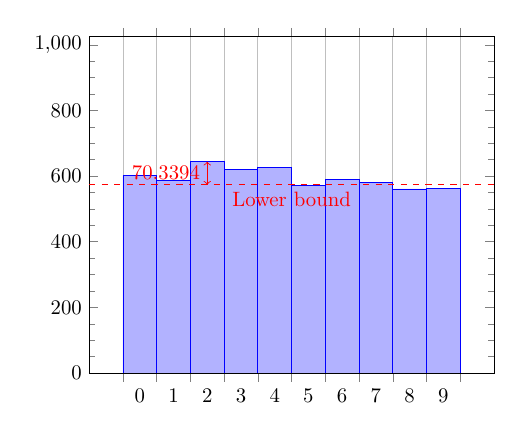
\begin{tikzpicture}[scale=0.75]
  \begin{axis}[ybar interval, ymax=1024.5,ymin=0, minor y tick num = 3]
    \addplot coordinates { (0,602.402) (1,586.819) (2,643.921) (3,618.819) (4,624.811) (5,572) (6,589.205) (7,579.157) (8,560.764) (9,563.197) (10, 465.681) };
\draw [red, dashed] ({rel axis cs:0,0}|-{axis cs:0,573.582}) -- ({rel axis cs:1,0}|-{axis cs:10,573.582}) node [pos=0.5, below] {Lower bound};
\draw [red, <->] ({axis cs:2.5,573.582}) -- ({axis cs:2.5,643.921}) node [pos=0.5, left] { 70.3394};
  \end{axis}
\end{tikzpicture}
\caption*{Weights repartitions on the first tree}
\end{minipage}
\begin{minipage}{0.49\textwidth}
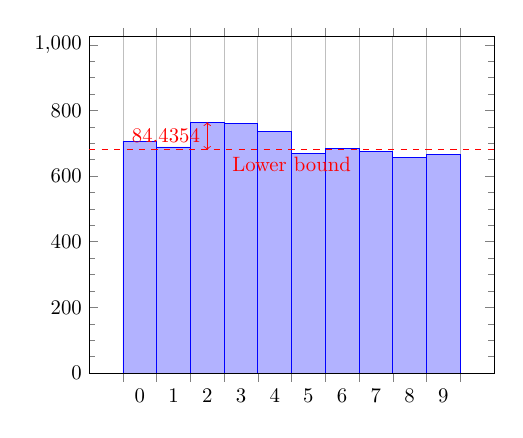
\begin{tikzpicture}[scale=0.75]
  \begin{axis}[ybar interval, ymax=1024.5,ymin=0, minor y tick num = 3]
    \addplot coordinates { (0,706.795) (1,688.63) (2,764.189) (3,760.535) (4,734.709) (5,669.024) (6,683.709) (7,674.457) (8,656.992) (9,665.669) (10, 465.681) };
\draw [red, dashed] ({rel axis cs:0,0}|-{axis cs:0,679.754}) -- ({rel axis cs:1,0}|-{axis cs:10,679.754}) node [pos=0.5, below] {Lower bound};
\draw [red, <->] ({axis cs:2.5,679.754}) -- ({axis cs:2.5,764.189}) node [pos=0.5, left] { 84.4354};
  \end{axis}
\end{tikzpicture}
\caption*{Weights repartitions on the last}
\end{minipage}
\begin{minipage}{0.49\textwidth}
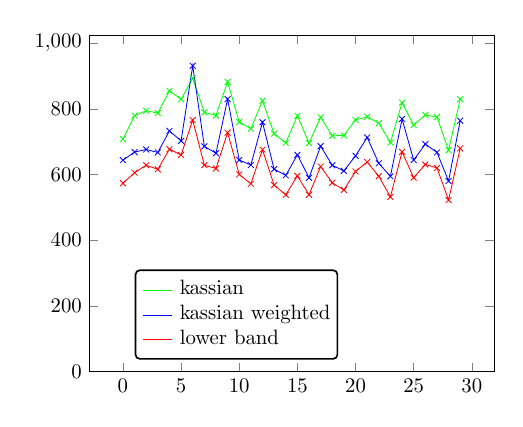
\begin{tikzpicture}[scale=0.75]
  \begin{axis}[ymax=1024.5,ymin=0]
    \addplot[color=green, mark=x] coordinates { (0,707.811) (1,779.441) (2,794.622) (3,787.535) (4,855.102) (5,829.394) (6,893.646) (7,789.63) (8,779.874) (9,882.449) (10,760.362) (11,739.701) (12,824.898) (13,724.591) (14,696.614) (15,779.134) (16,696.118) (17,774.598) (18,718.26) (19,719.087) (20,766.575) (21,776.22) (22,756.724) (23,697.756) (24,819.094) (25,750.827) (26,781.866) (27,775.055) (28,674.37) (29,829.551) };
    \addplot[color=blue, mark=x] coordinates { (0,643.921) (1,668.528) (2,676.504) (3,667.37) (4,733.079) (5,702.646) (6,931.362) (7,685.811) (8,665.094) (9,830.102) (10,644.339) (11,629.173) (12,759.512) (13,616.543) (14,597.488) (15,660.039) (16,590.339) (17,686.614) (18,628.37) (19,611.37) (20,657.055) (21,713.055) (22,634.173) (23,594.701) (24,769.496) (25,644.213) (26,692.787) (27,667.551) (28,580.362) (29,764.189) };
    \addplot[color=red, mark=x] coordinates { (0,573.582) (1,605.77) (2,628.569) (3,615.987) (4,677.332) (5,659.774) (6,766.106) (7,628.75) (8,618.558) (9,727.522) (10,600.557) (11,572.006) (12,675.985) (13,568.039) (14,538.254) (15,596.077) (16,538.542) (17,624.55) (18,574.913) (19,553.252) (20,609.639) (21,638.263) (22,594.901) (23,532.135) (24,669.126) (25,590.734) (26,630.754) (27,620.239) (28,522.412) (29,679.754) };
\node[draw=black,thick,rounded corners=2pt,above right=2mm] at (0, 0) {%
  \begin{tabular}{@{}r@{ }l@{}}
    \raisebox{2pt}{\tikz{\draw[green] (0,0) -- (5mm,0);}}&kassian\\
    \raisebox{2pt}{\tikz{\draw[blue] (0,0) -- (5mm,0);}}&kassian weighted\\
    \raisebox{2pt}{\tikz{\draw[red] (0,0) -- (5mm,0);}}&lower band
  \end{tabular}};
\end{axis}
\end{tikzpicture}
\caption*{ Per tree, maximum weights with kassian and our algorithm, and lower band }
\end{minipage}
